% ========== KRONSPIDSHJORT ==========
\begin{frame}{%
  \begin{minipage}[c]{0.30\textwidth}
    Kronspidshjort
  \end{minipage}%
  \hfill
  \begin{minipage}[c]{0.45\textwidth}
    \footnotesize
    \textbf{Jagttid:} 1.\ september -- 31.\ januar
  \end{minipage}%
  \hfill
  \begin{minipage}[c]{0.15\textwidth}
    \noindent\raggedleft
    
\includegraphics[width=0.5cm, height=0.5cm, keepaspectratio]{Billeder/Ikoner/star.png}%
    \hspace{0.2em}%
    
\includegraphics[width=0.5cm, height=0.5cm, keepaspectratio]{Billeder/Ikoner/star.png}%
    \hspace{0.2em}%
    
\includegraphics[width=0.5cm, height=0.5cm, keepaspectratio]{Billeder/Ikoner/star.png}
  \end{minipage}%
}
  \vspace{0.25em}
  \begin{columns}[T]
    % --- Venstre kolonne: Tekst ---
    \column{0.45\textwidth}
    \setlength{\parskip}{0.4em}
    \tiny
    \RaggedRight
    \textbf{\textit{Cervus elaphus}} – kronhjort i sit andet leveår. Kaldes spidshjort, fordi geviret typisk kun består af to enkelte spidser. \par
    \textbf{Udseende:}\\
    \quad – To enkle gevirstænger uden forgrening \\
    \quad – Mindre og slankere end ældre hjort \\
    \quad – Gult spejl der går op på ryggen \par
    \textbf{Levesteder:} Store skovområder. Kræver meget ro. Nataktiv og opholder sig i tæt vegetation om dagen. \par
    \textbf{Føde:} Lyng, græs, lav, landbrugsafgrøder, skud fra buske/træer. \par
    \textbf{Udbredelse:} Jylland og Sjælland. \par
    \textbf{Parring/brunst:} September/oktober. \par
    %\textbf{Forplantning:}\\
    %\quad – \textbf{Kønsmoden:} 1 år \\
    %\quad – \textbf{Mono/polygam:} Polygam \\
    %\quad – \textbf{Bestandsomsætning:} Langsom \\
    %\quad – \textbf{Kuld:} 1 kalv, sjældent 2 \par
    %\textbf{*Bemærk:} Mange lokale jagttider.
    % --- Højre kolonne: Større billede ---
    \column{0.52\textwidth}
    \centering
    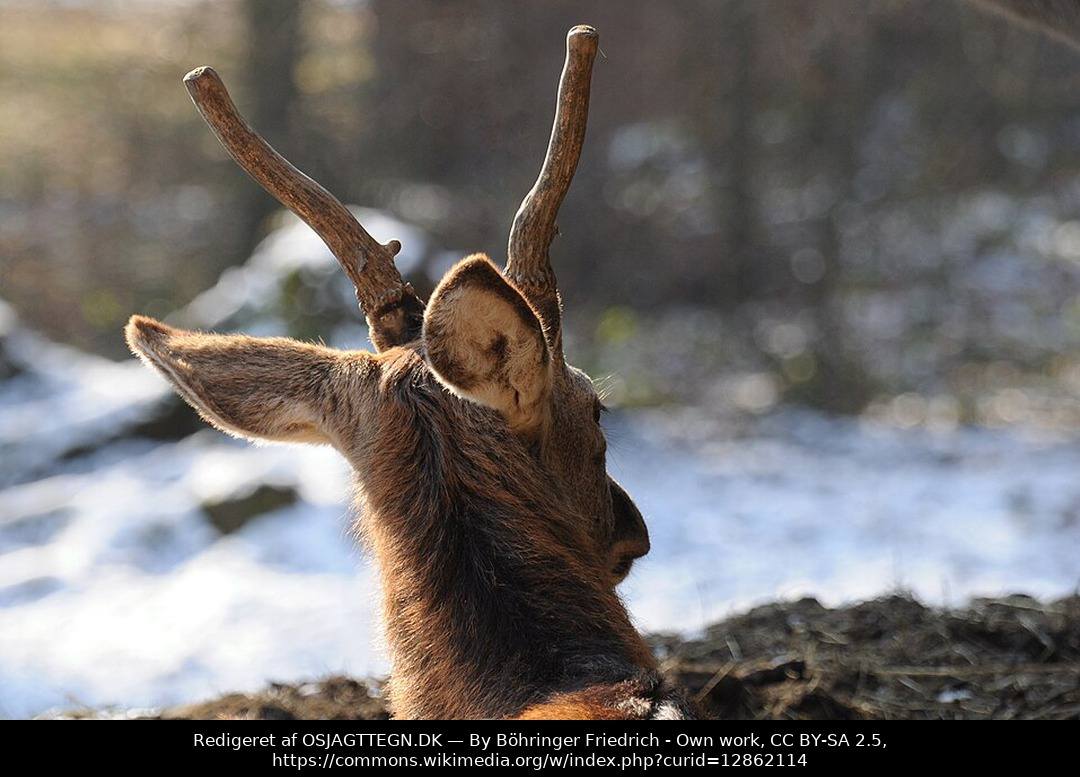
\includegraphics[width=\linewidth, height=7.2cm, keepaspectratio]{Billeder/Dyr/Pattedyr/hovdyr/kronvildt/kronspidshjort/kronspidshjort-01.JPG}
  \end{columns}
\end{frame}